\documentclass[]{article}
\usepackage[english]{babel}
\usepackage[explicit]{titlesec}
\usepackage{graphicx}

%opening
\title{Distributed Systems: Java RMI report}
\author{Tobias De Locht, Dries De Backker}
\date{3 November, 2017}

\begin{document}

\maketitle

\section{Design decisions}
When starting up the rentalserver, it's main method creates a new namingService object. This object is mainly responsible for registering car rental companies and looking up their objects by name. The main method also creates a new remotely accessible sessionManager object. This object is in charge of creating new sessions for clients as well as managers. So two type of session classes are available with each it's corresponding remote interface class. 
\\
The manager sessions are stateless while the reservation sessions are stateful. The reservation sessions are used by clients to check car availabilities and make or cancel reservations. The responsibilities of the manager is registering companies and obtaining statistics about the rental companies. TODO: life cycle van de sessions?

 
\section{Remote objects}

TODO: welke objecten zijn remote en waarom? welke objecten moeten hierdoor serializable zijn? Welke objecten zijn geregistreerd in de RMI registry en waarom? welke remote objecten zijn gelocaliseerd op dezelfde host en waarom?
\section{Synchronization}
TODO:synchronization
\clearpage
\section{Diagrams}
{\begin{figure}[h]
		\caption{Class Diagram}
		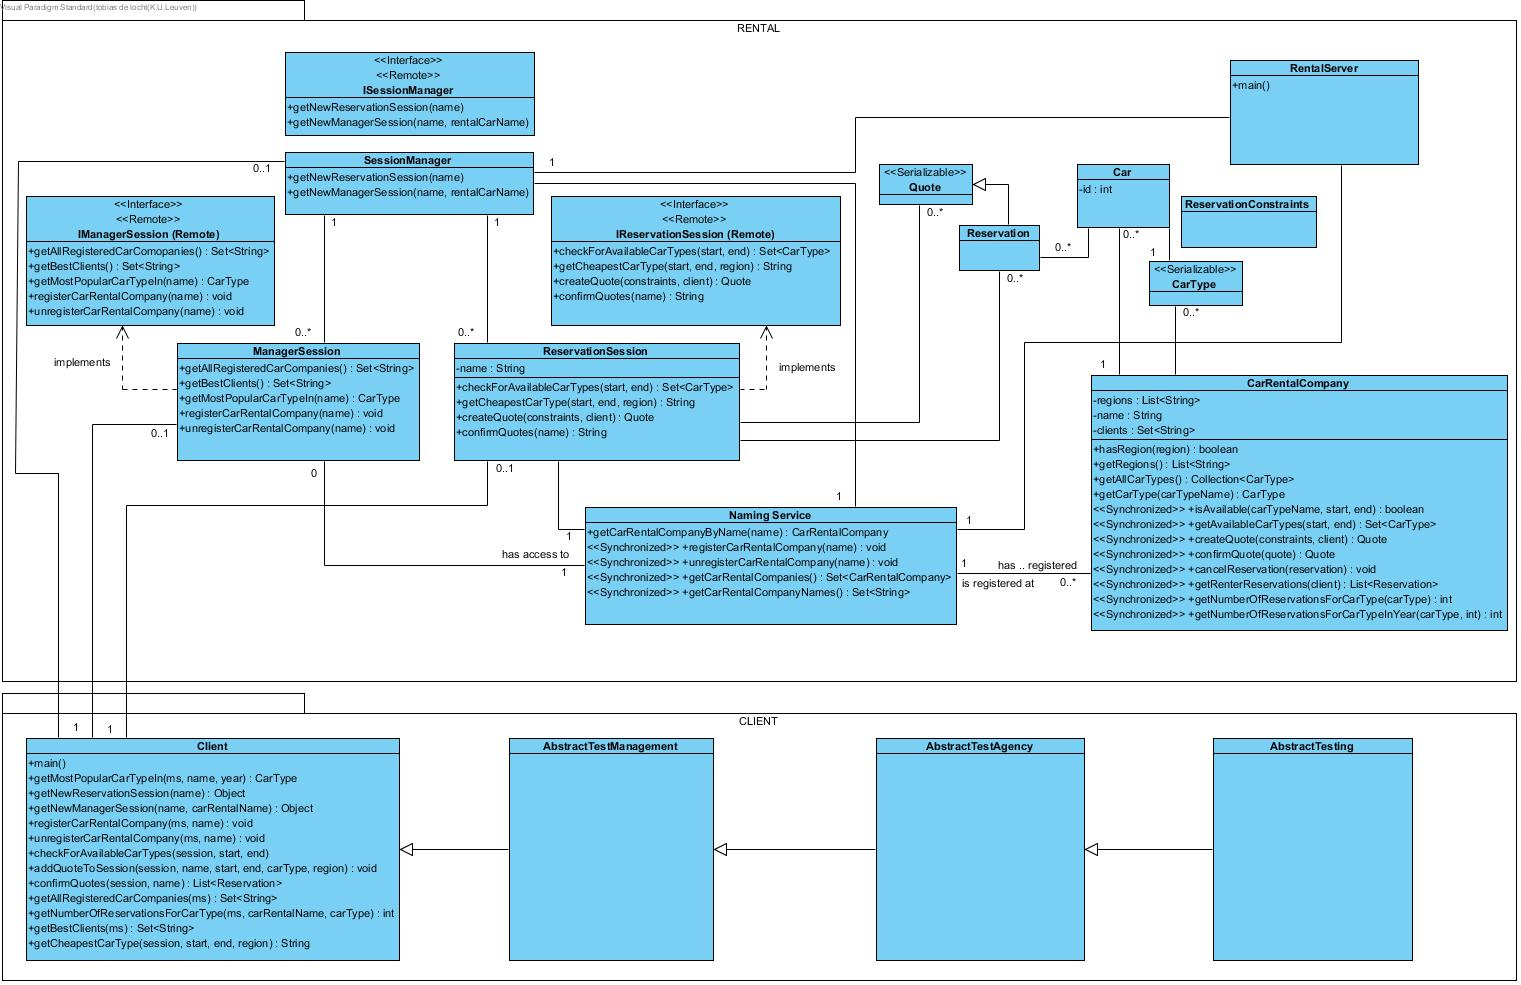
\includegraphics[width=1\textwidth]{classdiagram}
		\label{fig:class}
	\end{figure}
\clearpage
{\begin{figure}[h]
		\caption{Client session creation}
		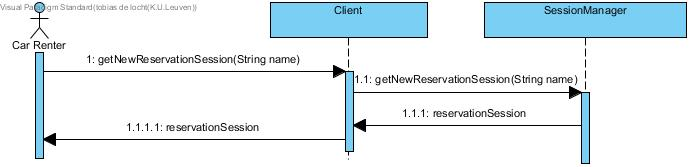
\includegraphics[width=1\textwidth]{clientseq}
		\label{fig:client}
	\end{figure}
{\begin{figure}[h]
		\caption{Reservation}
		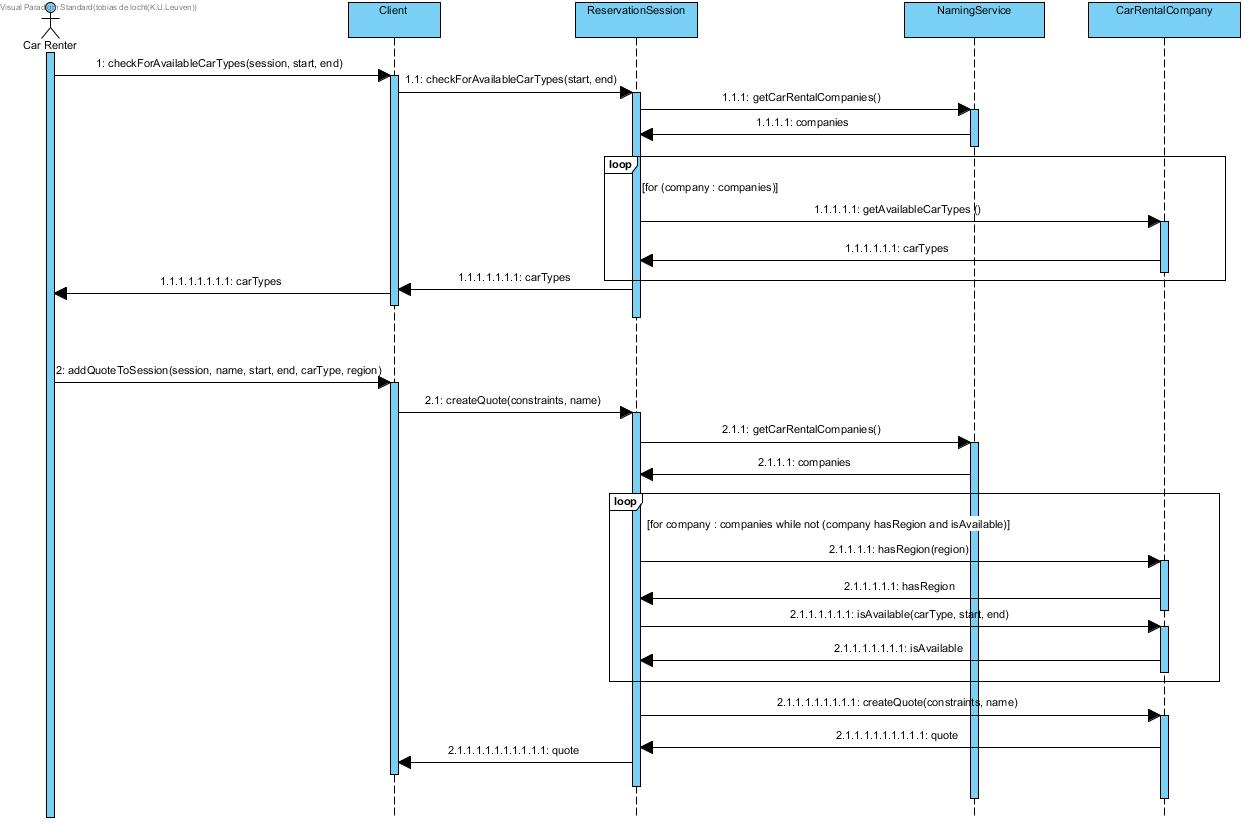
\includegraphics[width=1\textwidth]{reservationseq}
		\label{fig:reservation}
	\end{figure}
\clearpage
{\begin{figure}[h]
		\caption{Deployment}
		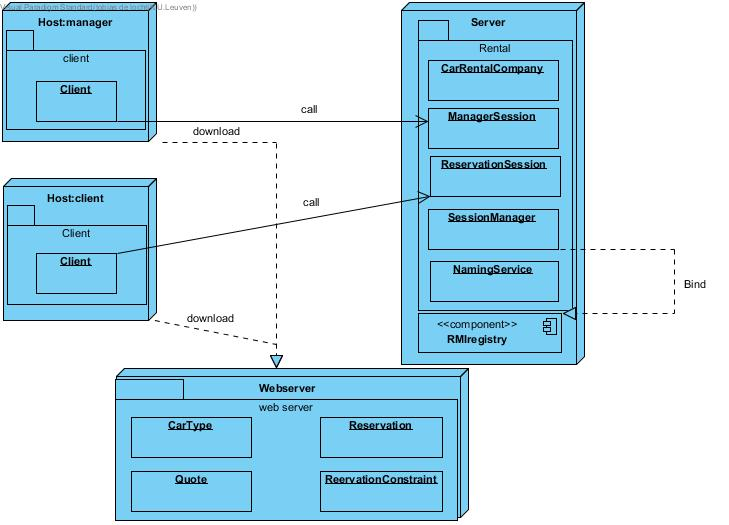
\includegraphics[width=1\textwidth]{deployment}
		\label{fig:dep}
	\end{figure}
\end{document}

